\usepackage{booktabs}%! Author = lazza
%! Date = 11/04/2022

\section{Pipelining}\label{sec:pipeline}

MIPS instructions
\subsection{MIPS}\label{subsec:heterogeneous-systems}
The MIPS architecture is based on the SIMD model.
\begin{figure}
    \centering
    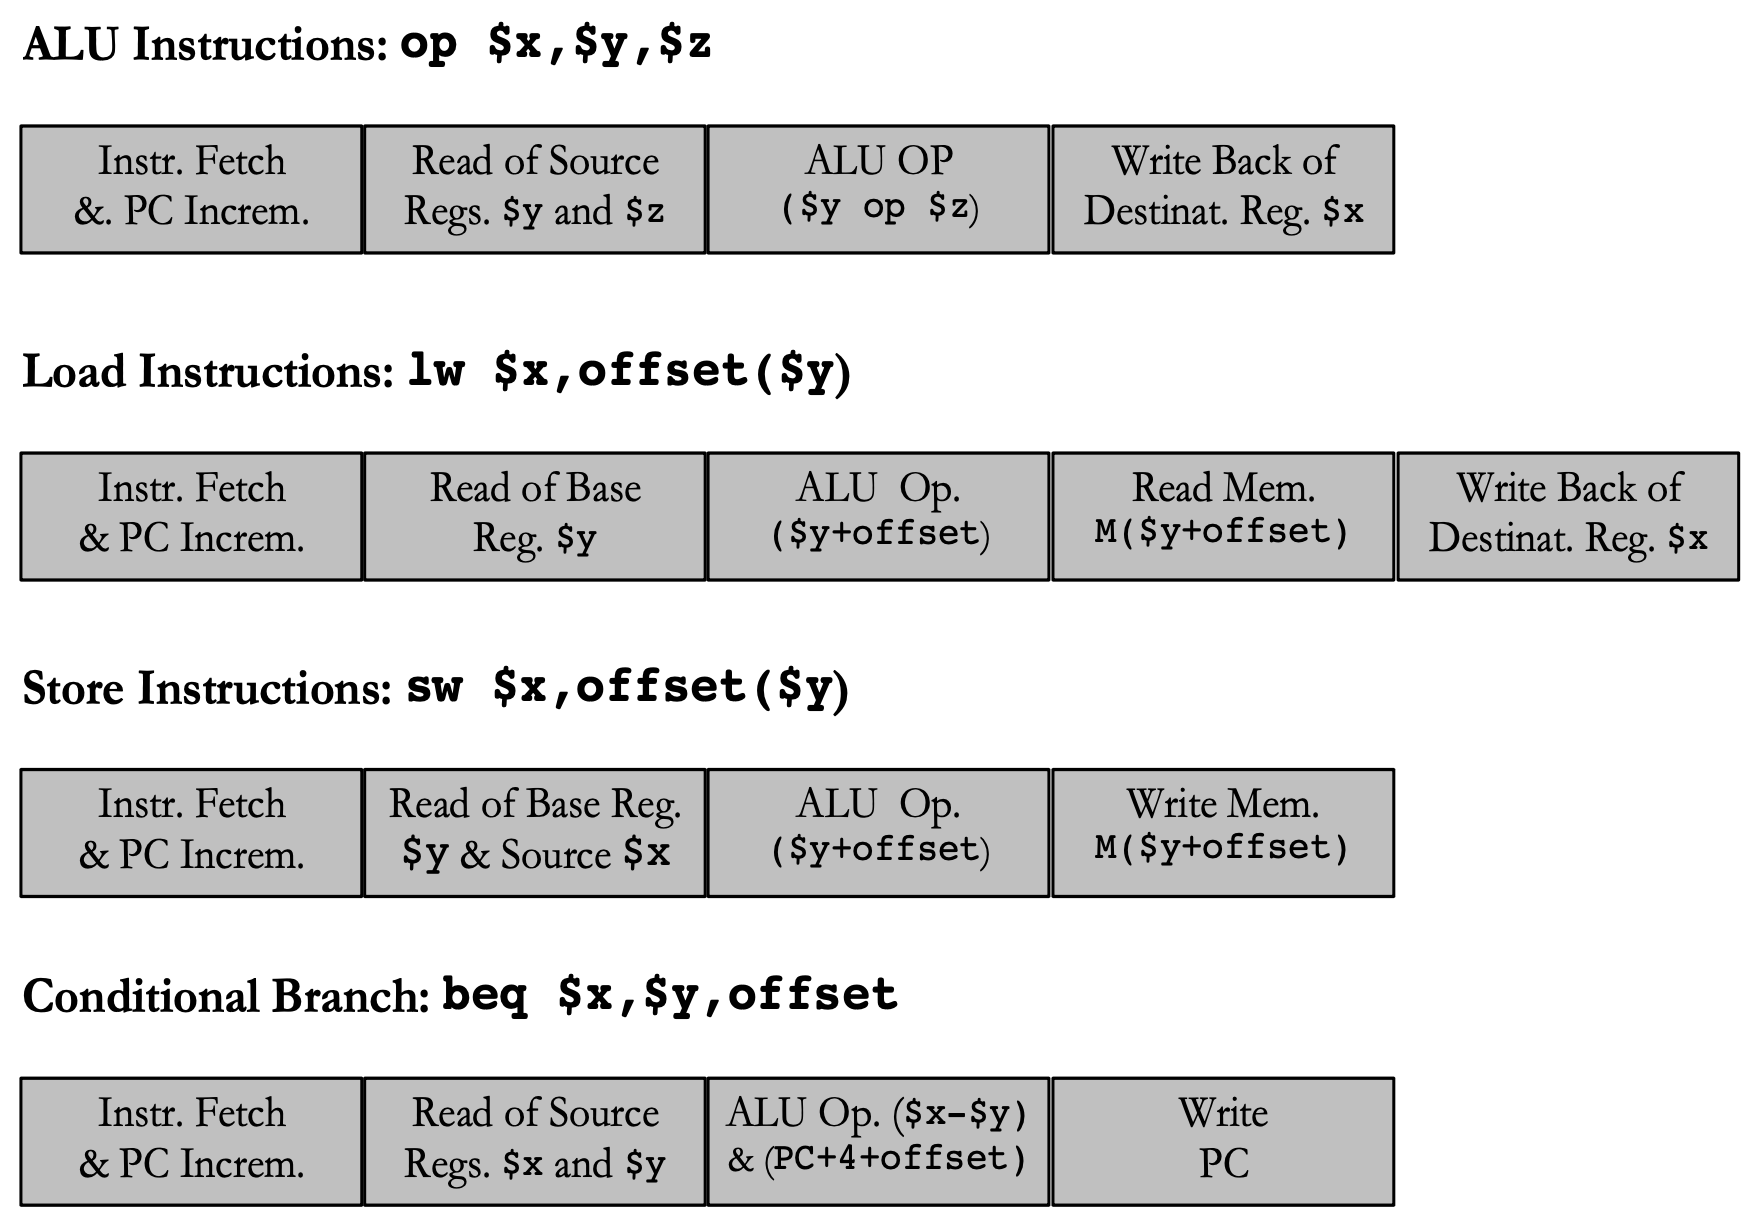
\includegraphics{images/MIPS-instructions}
    \caption{MIPS instructions}
    \label{fig: MIPS instructions}
\end{figure}
Instruction set, 32 bit
architecture specific

Exam:
- assembly --> specific instruction for an architecture
- design architecture

CPU = data path plus  control unit
Bus:
- control
- data
- address
Memory

pipeline multi-cycle process: latency vs throughput

RF : Register file is used in ID and WB phase, clock divided in rising edges and falling edge, sometimes there
are dependencies among instructions

Register File used in 2 stages: Read access during ID and write access during WB
– What happens if read and write refer to the same register in the same clock cycle?
• It is necessary to insert one stall
• OptimizedPipeline:the RF read occurs in the second half of clock cycle and the RF write in the first half of clock
cycle
– What happens if read and write refer to the same register in the same clock cycle?
• It is not necessary to insert one stall

\subsection{Hazards}\label{subsec:hazards}
A hazard is created whenever there is a dependence between instructions, and instructions are close enough that the
overlap caused by pipelining would change the order of access to the operands involved in the dependence.
Hazards prevent the next instruction in the pipeline from executing during its designated clock cycle.
Hazards reduce the performance fromthe ideal speedup gained by pipelining.

\subsubsection{Structural hazards}
Use of the same resource from different instruction simultaneously.
No structural hazards in MIPS architecture:
– Instruction Memory separated from Data Memory
– Register File used in the same clock cycle: Read access by an instruction and write access by another instruction

\subsubsection{Data Hazard}
Attempt to use a result before it is ready

-RAW
Techniques: design (compilation-time) and hardware solutions (run-time)

Compilation Techniques:
– Insertion of nop (no operation) instructions
– Instructions Scheduling to avoid that correlating instructions are too close
    • The compiler tries to insert independent instructions among correlating instructions
    • When the compiler does not find independent instructions, it insert nops.
Hardware Techniques:
– Insertion of “bubbles” or stalls in the pipeline
– Data Forwarding or Bypassing

insertion of nops (no operation), compiler
insertion of bubbles, architecture

scheduling, reordering instruction without changing the overall result

forwarding, shortcutting data from origin to next use EX-EX path, MEM-EX path, MEM-ID path, in WB-ID there's no
need for a path, just persistence trough clock cycle.

-Load/Use hazard, it requires a stall to use the MEM-EX path, two stalls to use the optimized pipelining

-Load/Store hazard, forwarding MEM-WB

MEM-ID path is not useful if we divide clock cycle in rising and falling edge

Other architecture different from 5 stage mips:
-WAW write after write , conflict if write after write are not executed in order
-WAR write after read

Data hazards: RAW(dependency), WAW, WAR(anti-dependency)
immagine slide 17 introilp_v2

\subsubsection{Control hazards}
Attempt to make a decision on the next instruction to execute before the condition is evaluated.
Mux output based on ALU output.
Until alu doesn't compute output PC is not known, we cant know the next instruction.

PC available at the memory stage.

Generally true statements are executed during the waiting for the next instruction, as if the condition is true, just PC plus 1, and then see if the branch is taken.

branch stall with and without forwarding, 3 vs 2 stalls

additional solution is the early evaluation of the PC, new pipeline in witch PC adder is anticipated in the ID stage, 1
stall to fetch the correct instruction

This solution bring an issue with RAW: we do have to insert a stall.

Branch prediction techniques
- static (compile-time)
branch always not taken, no jump
branch always taken, always jump, not always good because we have to calculate BTA branch target address (Mips pipeline)
backward taken forward not taken, loop taken, if not taken
profile-driven prediction, we are going make several runs of our program and the choice is based on statistical data
delayed branch, rescheduling an independent instruction (also from the branch):
    from before (no penalty in mips)
    from target
    from fall-through


- dynamic (run-time)
Branch outcome predictor, to predict the direction of a branch (i.e., taken or not taken).
save the outcome value, i.e,

Branch target predictor, to predict the branch target address in case of taken branch
Save BTA info in a target buffer that  we will use if we take the branch, save the target address.


Branch History Table (or Branch Prediction Buffer) - outcome predictor
Table containing n-bit for each entry that says whether the branch was recently taken or not.
Table indexed by the lower portion of the address of the branch instruction.
slide 11:
n-bits branch store address
k-bits to index the branch addresses in the buffer, 2^k entries
last k-bits of branch store address may collide!

1-bit branch history table
1-bit for each entry says whether the branch was recently taken or not.
Till now we have a profile driven prediction, dynamic element is the update the value based on past instruction
Example:
0, prediction not taken, outcome not taken - no update
0, prediction not taken, outcome taken - update 0 to 1
0, prediction taken, outcome not taken - update 1 to 0
see automata slide 28

A misprediction occurs when:
– The prediction is incorrect for that branch, or
– The same index has been referenced by two different branches, and the previous history refers to the other branch.
    • To solve this problem it is enough to increase the number of rows in the BHT or to use a hashing function (such as in GShare).

2-bit branch history table
The prediction must miss twice before it is changed.
In a loop branch, at the last loop iteration,we do not need to change the prediction.
For each index in the table, the 2-bits are used to encode the four states of a finite state machine.
see automata, 4 states, 2 bits
do exercise slide 74

n-bit branch history tables
best one is 2-bit

correlating branch predictors
(m,n), best one is (2,2)



\section{Exercise session 1 - Data Hazards}\label{sec:exercise-session-1}
IF instruction fetch - ID instruction decode - EX execution - MEM memory access - WB write back

single fetch per clock cycle : Microprocessor without Interlocked Pipelined Stages (SIMD)

data conflict vs data hazards?
A conflict can be an hazard

exercise1:
- highlight conflicts
- data path, introduce forwarding, memorize data path + 3 forwarding path (diagonal) + 1 forwarding in the same clock
- rescheduling

exercise2:
- highlight conflicts
Resolve data hazards
- without forwarding, stalls
- with forwarding
- scheduling
Resolve control hazards
- apply backward taken forward not taken

Problem:
solution a
\[CPI = \frac{clock cycles}{instruction} = \sum_{i=0}^{n} CPI_i \times F_i\]
where \(F_i = \frac{I_i}{Instruction count}\)

solution b,c,d vedo formulario


\section{Exercise session 2}\label{sec:exercise-session-2}
Performance analysis

Throughput vs Response time (latency?)
- faster hardware : more throughput and minor response time
- adding parallel hardware: more throughput

Amdahl's law
1) Hardware : Enhance fraction (of our application, program), if we enhance the entire application the max overall
speedup is = 2,86.

2)Parallelism: strong scaling, #thread vs serial part of a program
Power consumption?

3) pipelining
conflict = dependency != hazard

4) dynamic branch prediction


\section{Instruction level parallelism}\label{sec:instruction-level-parallelism}
Definition: potential overlap of execution among unrelated instructions
Overlapping possible if:
- no structural hazards
- no raw, war, waw stalls
- no control hazards

pipeline CPI

In mips the only possible structural hazards is WB-ID where the same resource/register can be accessed,
this issue is solved by splitting the clock cycle in rising edge (WB) and falling edge (ID).

WAR and WAW were not possible with ADD operation with integers, MULT and DIV use floating point numbers.
New stage introduced, it allows for multi-cycles - complex pipelining, problem synchronization, out-of-order write
hazards due to variable latencies of different FUs.

WB-ISSUE same cycle instead of WB-ID\@.
Multiple arrows entering the WB, variable latency can cause concurrent writes (besides out-of-order writes).

all functional units are pipelined!

learn assumptions<<

dependencies:
- data
- control
- name, WAR & WAW generated by the lack of registers

Techniques:
--> renaming
--> scheduling: static (compiler) and dynamic

-> superscalar



-----
Static scheduling and VLIM architectures

single core multi-cycle parallelism (till now)

CPI>1 possible with superscalar and VLIM
Very Long Instruction Words VLIW
(fixed number ofo instruction only in the slides)

multiple op per cycle - means op in the execution phase alu, operation != instruction

explicit parallelism - compiler based parallelism

single control flow - 1 program counter
multiple-issue = more than one instruction fetched per cycle


Exercise: given assembly code - schedule instructions (slide 35)
FP ops: floating point operations

Loop unrolling
non-FP ops can have multiple schedule locations, when not needed is it recommended using a new instruction

Software pipelining
loop = prolog + iterate + epilog

performance counts only the body (iterate), body of the loop dominates prolog and epilog.



Trace scheduler

Speculation and predication


Rotating Register Files

-----

Exercise session 3

a) mips pipeline
- calculate CPI, IC, MIPS
IC instruction count
MIPS million of instructions per second = Clock freq / (CPI * 10^6)

b) simple pipeline
- reschedule

c) simple pipeline
- forwarding

d) BHT 1-bit 2-bit
- colliding addresses


\subsection{Dynamic Scheduling}\label{subsec:dynamic-scheduling}

Scoreboard algo for dynamic scheduling

when is it safe to Issue an instruction slide 13
-
-
-
-

scoreboard manages commits to registers

RAW detected in ID stage, ID stage divided in two:
- instruction decode
- read registers

Scoreboard:
RAW ID stalls
WAR WB stalls
WAW not issued (stall the issue) - register renaming not used

techniques:
- register renaming

Scoreboard control structure:
1. instruction status, tells witch istr is being executed
2. functinal status, state of the functional unit
3. register result status, indicated which functional unit will write each register.

Qj and Qk tells who is going to provide the data in terms of functional unit (if not available yet)
Rj and Rk tells if the data is ready or not, prevents WAR

ADDD, DIVD, MULTD what D stands for?

in-order issue
out-of-order read
out-of-order write

-----

Tomasulo algo

load and store treated as integer FU

Common Data Bus - serialized access to write back
CDB provides values before they are saved into registers (somewhat similar to path forwarding)

FP floating point?

Reservation Station RS components
-
-
-
\ldots

STAGES
- issue
-
-

V value
Q pointer

LD: 1 cc to integer operation (offset + base address) and 1 cc to access the memory = 2 cc for Execution Completion + 1 cc to commit in the CDB

R(F4) = F4 value, register f4 Renamed

in-order issue
out-of-order execution
out-of-order write

try to do exercise on the slides

in case of concurrent writes choose the one that belongs to the critical path.

Scoreboard vs Tomasulo:
- structural hazards in scoreboard
- lack of forwarding in scoreboard


---

Exercise session 4

Complex Pipeline aka VLIw
- useful for FP operations (not considered in MIPS arch)
- different latency for different FU, we can reach the WB with different latency, out-of-order commit (WAW and WAR possibles)
- data and structural hazards? why structural? structural happens when two instruction need the same resource
in-order-issue in MIPS and VLIW,

FU units can be pipelined, example slide 13, DIV functional unit is multi-cycle and can't be pipeline, whereas the other
FU can be pipelined.

Complex pipeline assumption!
- in-order issue
- out-of-order commit

ese A) feasible solutions, problems:
1/4 out-of-order issue
2/4 structural hazards on c8 and c11, same resource WB is request by two instruction! (besides having data hazards)
3/4 structural hazard on C11
4/4 Feasible:
structural hazard on C11 solved by committing previous instruction and stalling 1 cycle the other.
RAW hazard solved by stalls on ISSUE stage, where we read the register (ID only decode now), IS and WB in the same cycle is OK\@.
WAR hazard instr 4 can enter the IS stage starting from cycle c7, which is WB stage (WB before or same cycle of IS) for instr 1
WAW same as before?

We cannot enter the issue stage if there's a WAR or WAW hazard until the WB stage.
Stalls for WAW and WAR need to wait in the ID stage, RAW in the IS stage, for no particular reason.

Adding buffer for instructions we stall only in the ISSUE stage letting IF and ID to not be stalled by structural hazards.

ese B) VLIW schedule
3-issue? what does that mean? maybe simultaneous issues

In clock C8 there is no WAR hazard since register 4 is read by the two instruction at the same time and then addi will overwrite
register 4  in the next instruction without compromising the other instruction.

bne instr is on cycle C10 because we need register 4 in ID stage to early evaluate the PC, so we need to leave C9 to ID.
(See exe 5, first exercise)

pipelined version of the exercise, easy.

ese C) VLIW schedule, fully pipelined


----

Exception handling

definitions
exception :
interrupt : external of internal event that needs to be processed by another program (the interrupt handler), at the end resume normal execution

External async events:
- input output device-request
- timer expiration
- power disruptions, hardware failure

Internal sync event:
- undefined opcode, privileged instruction
- arithmetic overflow, FPU exeception
- misaligned memory access
- virtual memory exceptions: page faults, TLB misse, protection violations
- traps: system calls, e.g., jumps into kernel

Exception classes:
- synchronous vs asynchronous, asynch caused by devices external to the CPU and memory and can be handled easily
- user requested vs coerced, user requested are predictable: treated as exceptions because they use the same mechanism that are used
to save and restore the state;
handled after the instruction has completed.
Coerced are caused by some HW event not under control of the program.
- user maskable vs user nonmaskable
- within vs between instructions
- resume vs terminate

For the exam study difference between pairs.

Invoking the interrupt handler:
- terminate exec of instr till PC-4
- store the PC in EPC register, exception program counter
- disable other interrupts and transfers control to a designated interrupt running in the kernel mode

In the cpu we have two modes: user-mode and kernel-mode (unstoppable).

precise interrupts
- easy handled

Exception handling in the 5-stage pipeline


----

Exercise session 5

tiny url - exercises

Branch always taken not very useful if early prediction is present.

a) Scoreboard
See recap about scoreboard

In case of feasible configuration question, if it is not feasible one reason suffices.
MULTF and MULTD are floating point, what's the difference?

WAW hazard prevents instruction to be issued, solved at the clock cycle after previous WB
WAR hazard stuck in the issue stage, solved at the clock cycle after previous WB

b) Complex pipeline (watch it again min 52) + branch prediction
Warning: store instruction just reads registers, no transitivity: indicate all possible conflicts

infinite buffer in the issue stage, RAW and stall happens in this stage.
WAW and WAR stalls in id stage till a clock cycle before WB, in WB the IS stage can start.

target address of branch available in the fetch stage

----

Tomasulo Loop

WAW and WAR solved by construction.
To issue an operation we have to check theres a Reservation Station available.

Load (issue stage clock):
- FU load1 busy "yes", address "offset+base addr"
- Reg Res Status "destination address" write FU operating the load, label not important (can use the name of the FU)

Mult (issue stage clock):
- FU mult1 busy "yes", Op "multd", Vj "", Vk "value available - copied (R)", Qj "resister result status pointer label to the data we need", Qk ""

Store (issue stage clock):
- FU store1 busy "yes", address "offset+base addr", FU "pointer label to the data we are waiting, e.g., mult1"

the renaming of the register creates a point to point connection between FU, creating a data flow

Important: in case of reduced loop (e.g., 2 cycles) write down that the loop is being iterated, although we are not seeing it during the exercise,
this means updating FU tables as well.

Data from a FU is available from the write result stage clock.

?? 1 SD has 18 as completion clock, 15+2cc = 17

The multiplications are overwriting registers



HW-based speculation